% ************************************************************************
%
% Automated Neuron Reconstruction from 3D Fluorescence Microscopy Images 
% using Sequential Monte Carlo Estimation
%
% ************************************************************************
\chpos{15mm}{8mm}
\chapter[Automated Neuron Reconstruction from 3D Fluorescence Microscopy Images using Sequential Monte Carlo Estimation]{Automated Neuron Reconstruction from 3D Fluorescence Microscopy Images using Sequential Monte Carlo Estimation}
\chaptermark{Automated Neuron Reconstruction using Sequential Monte Carlo Estimation}% from 3D Fluorescence Microscopy Images 
\label{ch4:pnr}

\myabstract{\lettrine{M}{icroscopic} images of neuronal cells provide essential structural information about the key constituents of the brain and form the basis of many neuroscientific studies. Computational analyses of the morphological properties of the captured neurons require first converting the structural information into digital tree-like reconstructions. Many dedicated computational methods and corresponding software tools have been and are continuously being developed with the aim to automate this step while achieving human-comparable reconstruction accuracy. This pursuit is hampered by the immense diversity and intricacy of neuronal morphologies as well as the often low quality and ambiguity of the images. Here we present a novel method we developed in an effort to improve the robustness of digital reconstruction against these complicating factors. The method is based on probabilistic filtering by sequential Monte Carlo estimation and uses prediction and update models designed specifically for tracing neuronal branches in microscopic image stacks. Moreover, it uses multiple probabilistic traces to arrive at a more robust, ensemble reconstruction. The proposed method was evaluated on fluorescence microscopy image stacks of single neurons and dense neuronal networks with expert manual annotations serving as the gold standard, as well as on synthetic images with known ground truth. The results indicate that our method performs well under varying experimental conditions and compares favorably to state-of-the-art alternative methods.}

\vspace{9em}
% ************************************************************************
\begin{publish}
	Based upon: M. Radojevi\'{c}, E. Meijering, ``Automated Neuron Reconstruction from 3D Fluorescence Microscopy Images using Sequential Monte Carlo Estimation'', \textit{Neuroinformatics}, \textit{submitted} %vol. 0, no. 0, pp.0-0, 2018.   
\end{publish}

\section{Introduction}
\label{sec:intro}
The brain is regarded as one of the most complex and enigmatic biological structures. Composed of an intricate network of tree-shaped neuronal cells \cite{ascoli2015trees}, together forming a powerful information processing unit, it performs a myriad of functions that are essential to living organisms \cite{kandel2000principles}. Obtaining a blue print of the architecture of this network, including the morphologies and interconnectivities of the neurons in various subunits, helps to understand how the brain works \cite{ascoli2002computational, donohue2008comparative, cuntz2010one}, including how  neurodegenerative disease processes alter its function. A key instrument in this endeavor is microscopic imaging, as it allows detailed visualization of neuronal cells in isolation and in tissue, thus providing the means to study their structural properties quantitatively \cite{senft2011brief}.

Quantitative measurement and statistical analysis of neuronal cell and network properties from microscopic data rely on the ability to obtain accurate digital reconstructions of the branching structures \cite{halavi2012digital} in the form of a directional tree of connected nodes \cite{ascoli2007neuromorpho}. The ever increasing amount of available image data calls for automated computational methods and software tools for this purpose, as manual delineation of neurons is extremely cumbersome even in single image stacks, and is downright infeasible in processing large numbers of images \cite{svoboda2011past, senft2011brief}. Automating neuron reconstruction requires solving fundamental computer vision problems such as detecting and segmenting tree-like image structures \cite{meijering2010neuron, donohue2011automated, acciai2016automated}. This is complicated by the large diversity of neuron types, imperfections in cell staining, optical distortions, inevitable image noise, and other causes of ambiguity in the image data. Consequently, with the current state-of-the-art, manual proof-editing of automatically obtained digital reconstructions is often necessary \cite{peng2011proof}. Recent international initiatives such as the DIADEM challenge \cite{gillette2011diademchallenge} and the BigNeuron project \cite{peng2015bigneuron, peng2015diadem2bigneuron} have catalyzed research in automated neuron reconstruction but have also clearly revealed that further improvement is still very much needed before computers can fully replace manual labor in performing this task.

With this paper we aim to contribute to the developments in the field by proposing a novel fully automated neuron reconstruction method based on probabilistic filtering techniques. Starting from seed points that have a high probability of being centered at neuronal branches, our method recursively traces these branches by sequential Monte Carlos estimation, using state transition and measurement models designed specifically for this purpose. This results in a series of possibly overlapping but probabilistically independent estimates of the branches, which are subsequently combined into a refined estimate of the actual branch centerlines using mean-shifting. We presented early versions of the method at conferences \cite{radojevic2015automated, radojevic2017neuron} and donated one implementation of it (named Advantra) for inclusion in the BigNeuron benchmarking study \cite{peng2015bigneuron, peng2015diadem2bigneuron}. Since then we have improved the method and its software implementation and have significantly extended its experimental evaluation. Here we provide a detailed description of the method, its implementation, and the experimental results, and show that it performs favorably compared to several state-of-the-art neuron reconstruction methods from the BigNeuron project as well as an alternative probabilistic method \cite{radojevic2017automated}. The source code of our software implementation will be released along with this paper.

\begin{figure*}[t!]
	\begin{tabular}{@{}c@{\hspace{0.008\textwidth}}c@{\hspace{0.008\textwidth}}c@{\hspace{0.008\textwidth}}c@{\hspace{0.008\textwidth}}c@{\hspace{0.008\textwidth}}c@{}}
		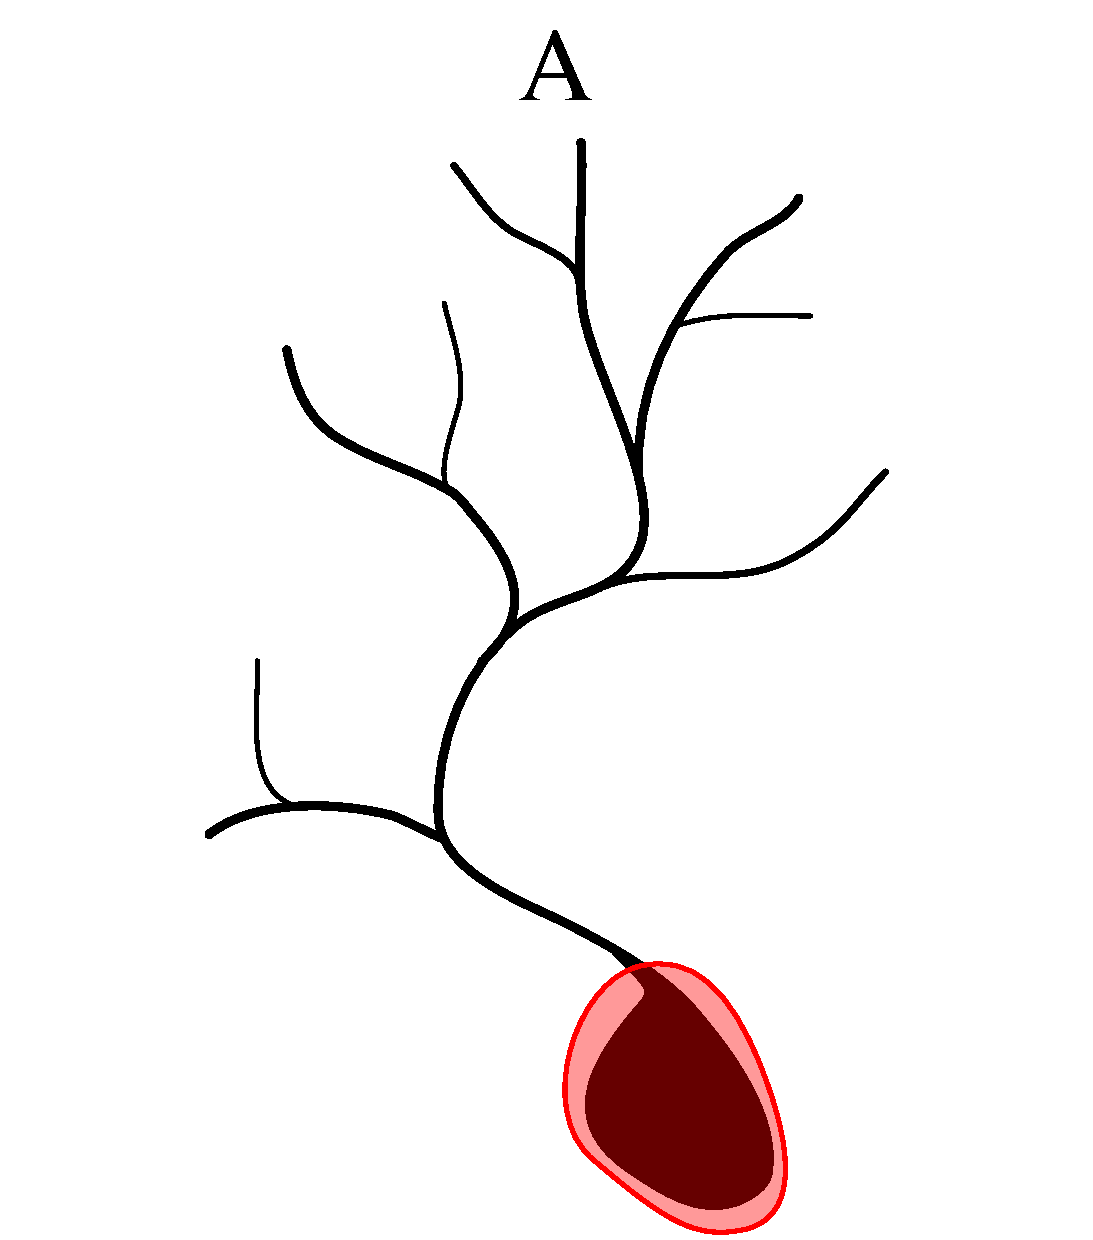
\includegraphics[width=0.16\textwidth]{./fig/method/A} &
		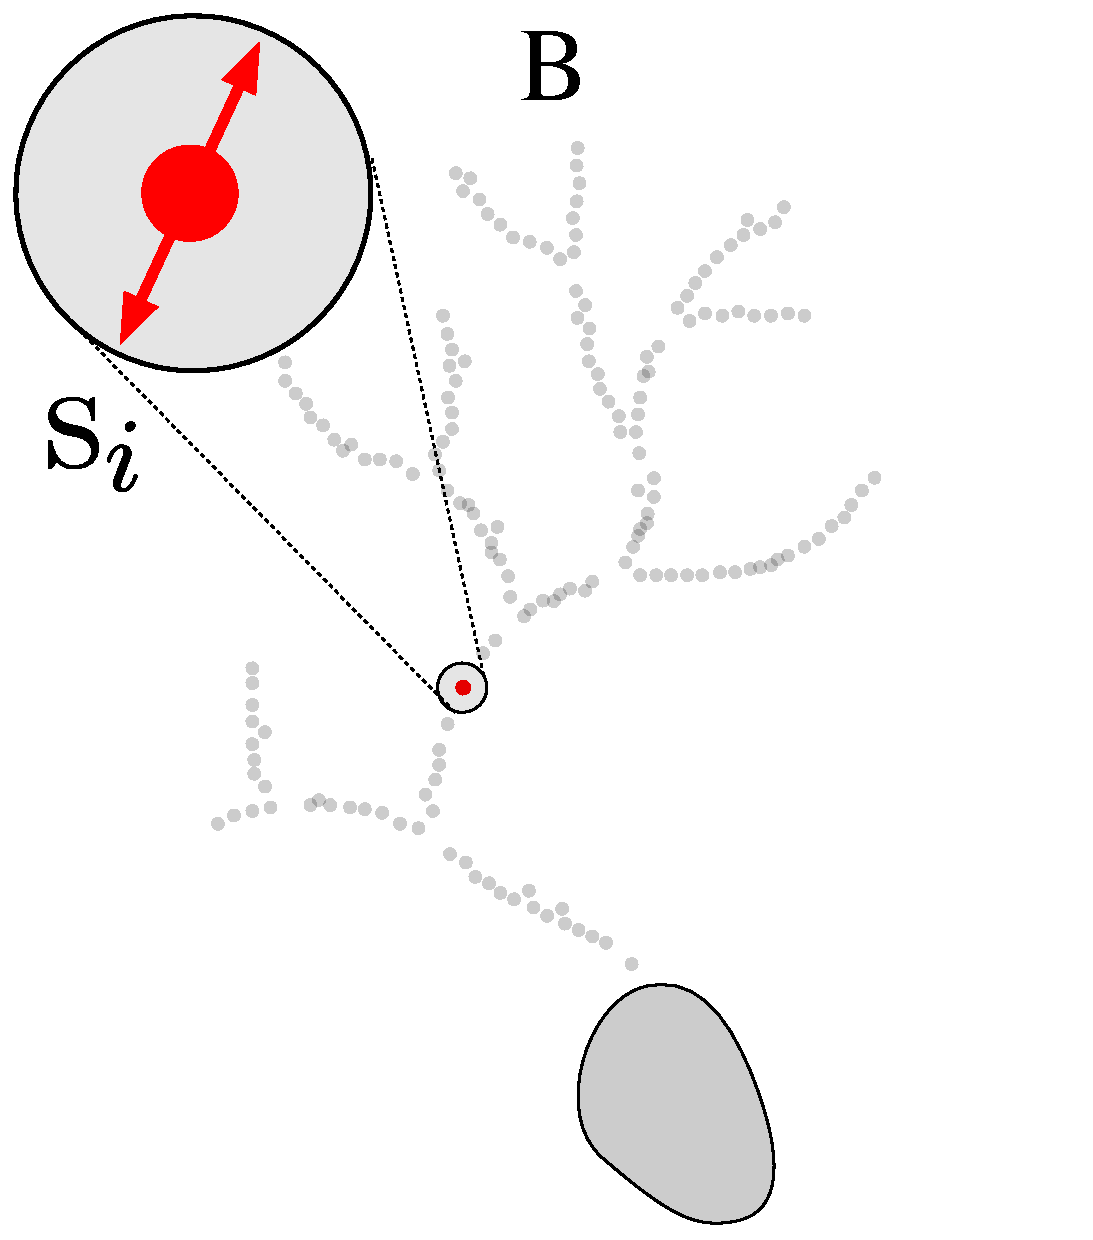
\includegraphics[width=0.16\textwidth]{./fig/method/C} &
		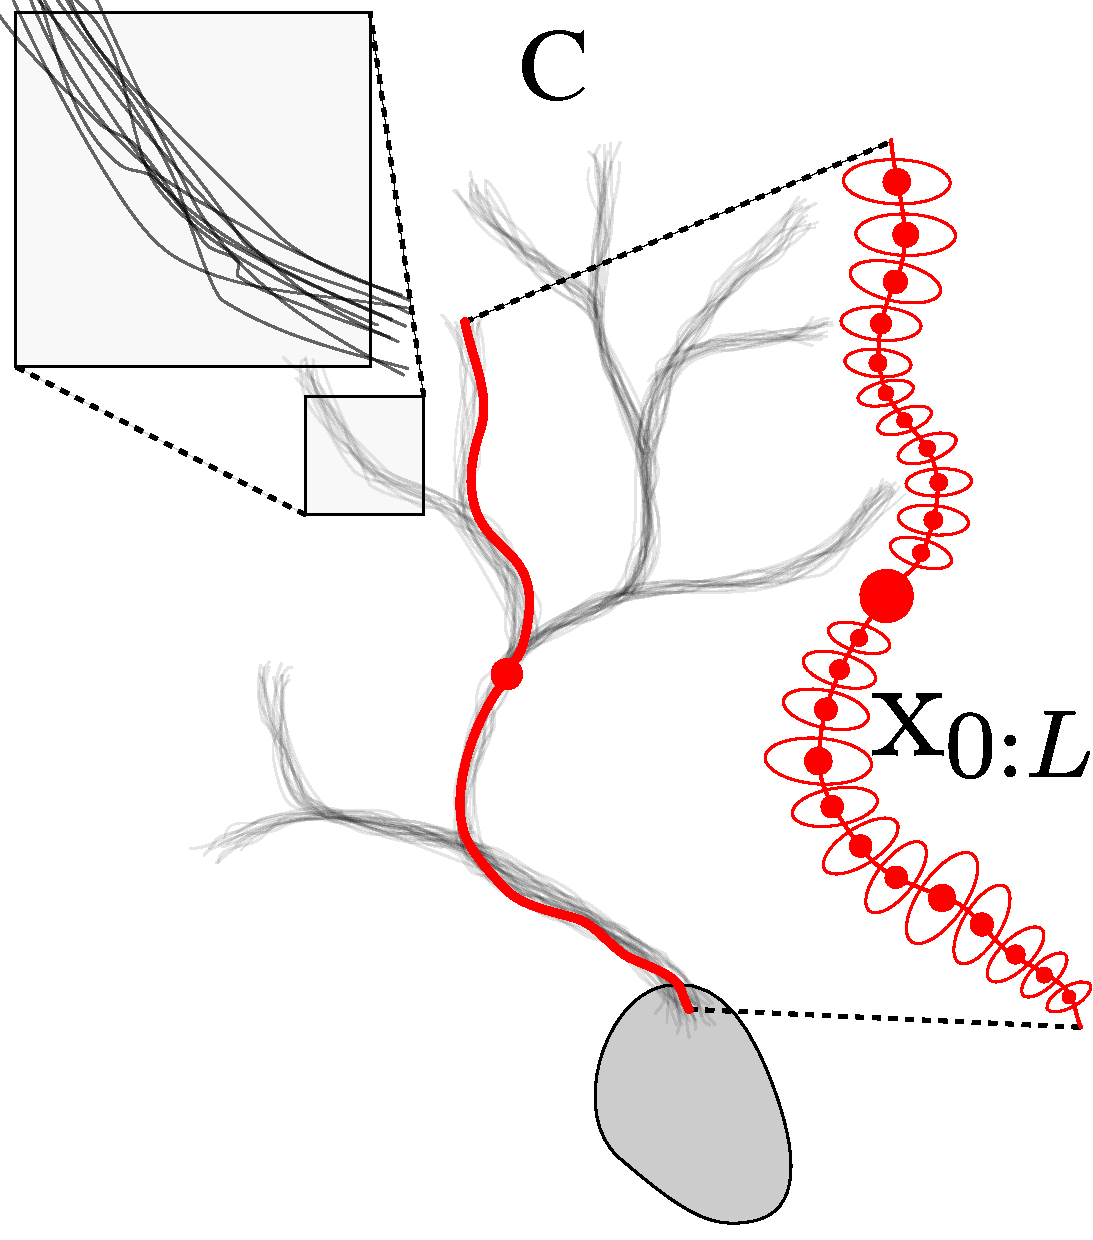
\includegraphics[width=0.16\textwidth]{./fig/method/D} &
		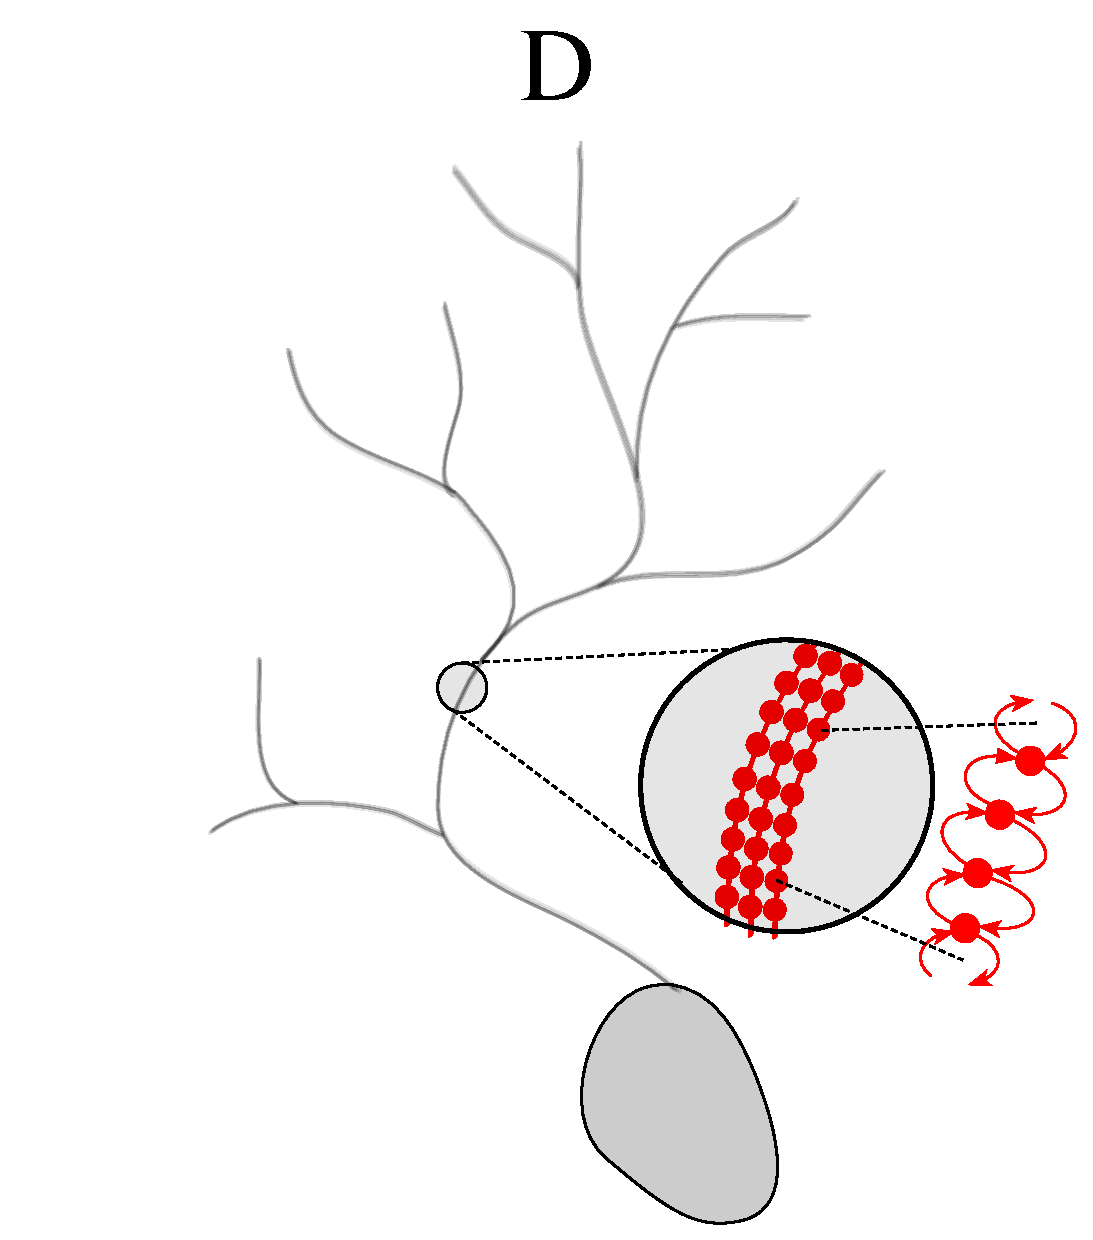
\includegraphics[width=0.16\textwidth]{./fig/method/E} &
		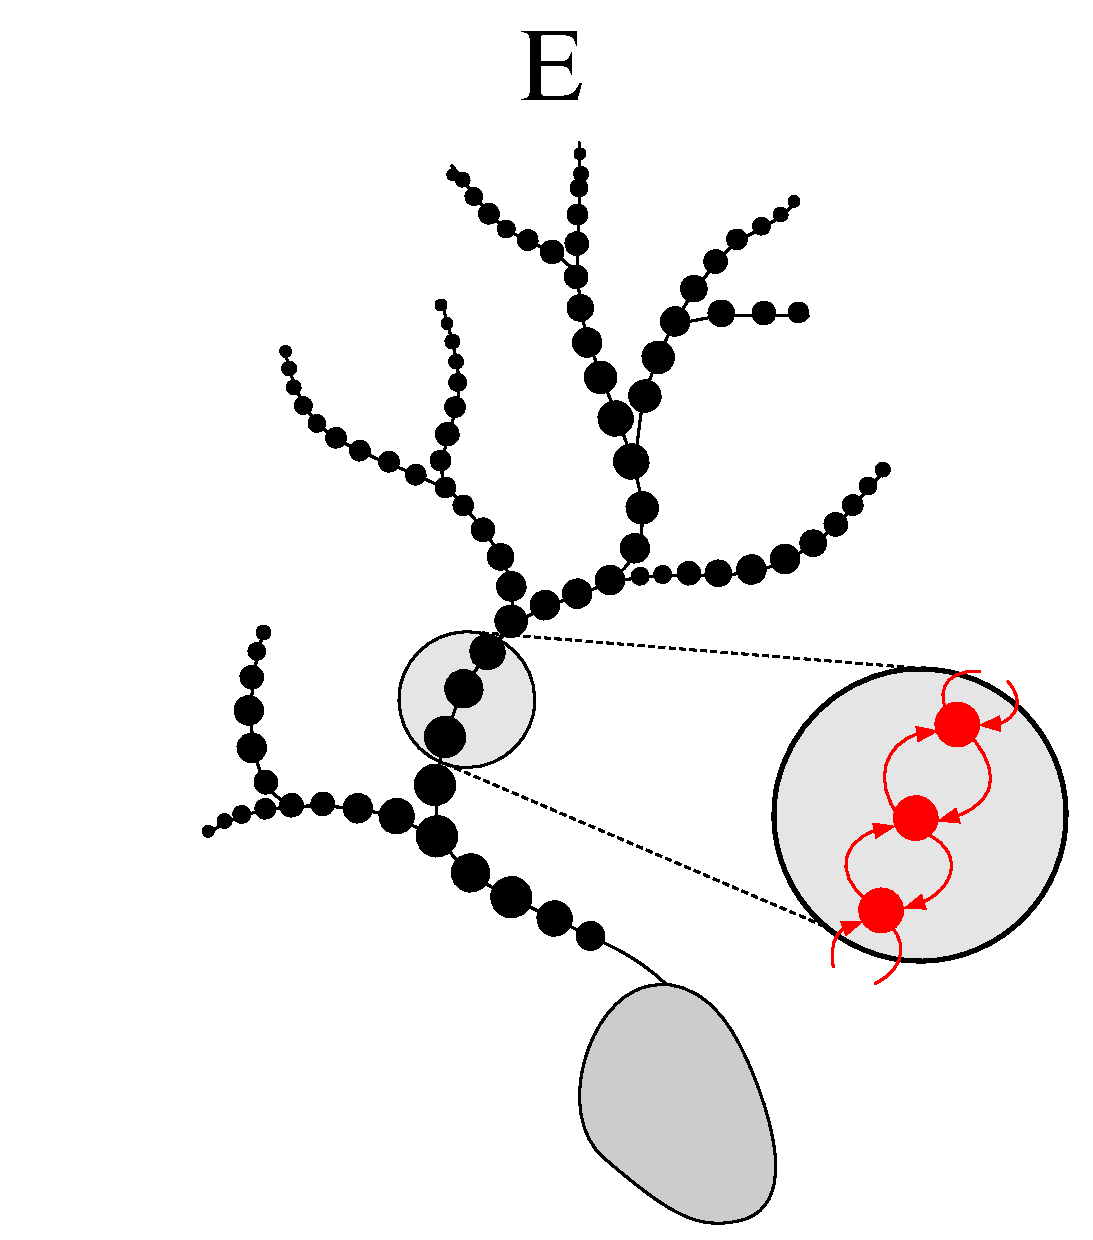
\includegraphics[width=0.16\textwidth]{./fig/method/F} &
		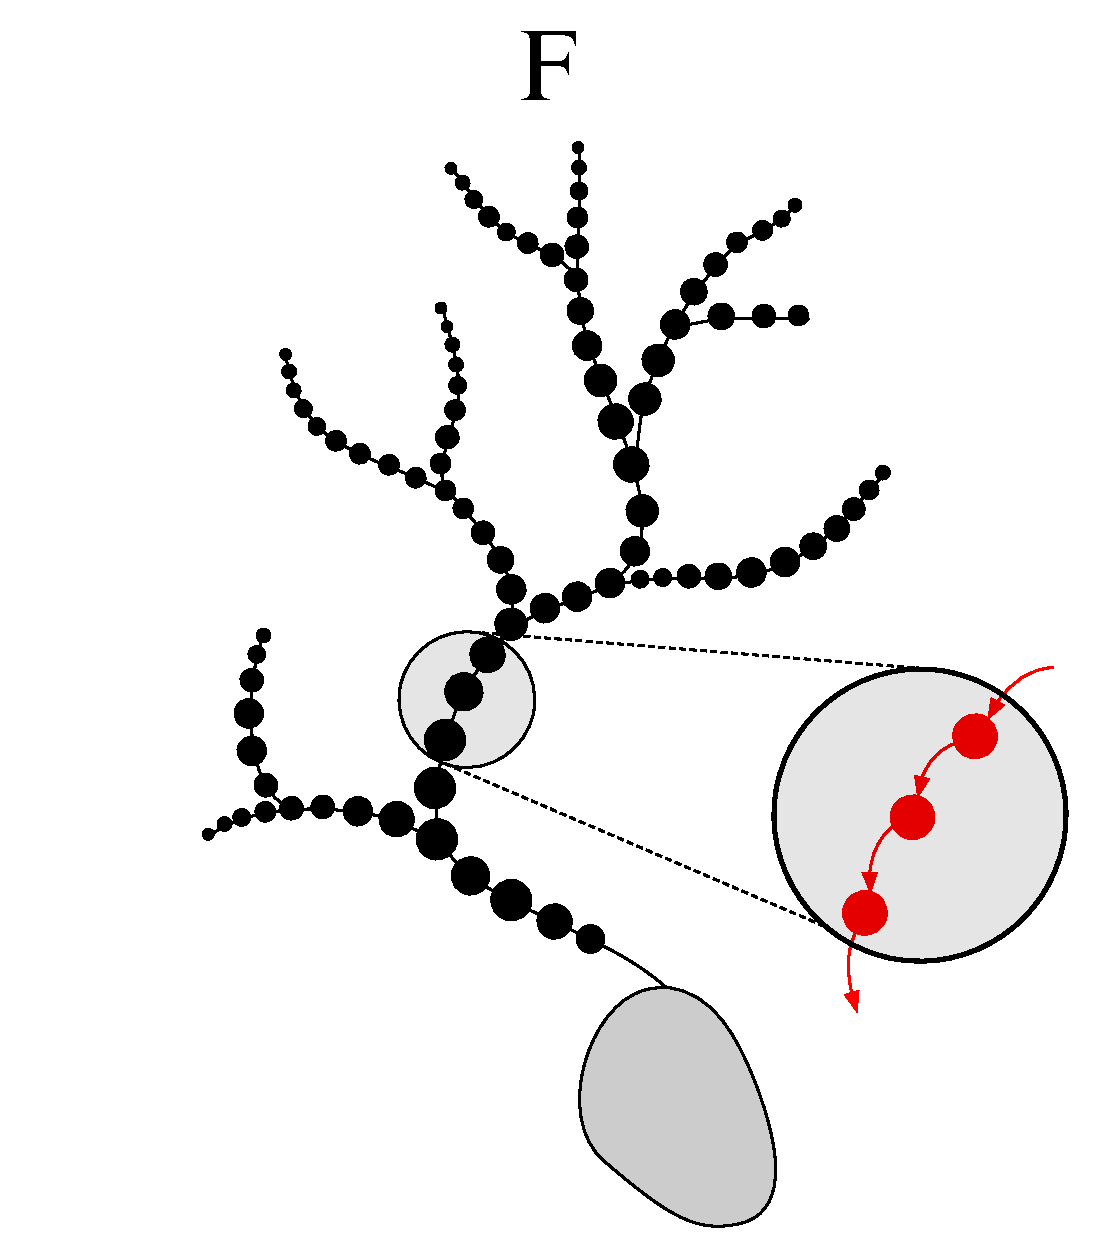
\includegraphics[width=0.16\textwidth]{./fig/method/G}
	\end{tabular}
	\caption{Schematic overview of the six main steps of the proposed method: (A) soma extraction, (B) seed extraction, (C) branch tracing, (D) trace refinement, (E) node grouping, (F) tree construction.}
	\label{fig:method}
\end{figure*}
